\chapter{Transforming Nonlinear Data with Logarithms}

\definecolor{kontinuablue}{HTML}{005892}

Certain relationships between two variables do not run in a straight line. Populations grow exponentially. Radioactive substances decay exponentially. When you try to fit a straight line to data like this, you may get a regression line, but the \textit{line of best fit} will be wrong or non-existent. Logarithm models can straighten out curved relationships, allowing you to use linear regression techniques on data that is not linear in its raw form.

\section{Exponential Models}

A content creator posts a video and tracks how many views it gets each day:

\begin{table}[H]
\centering
\begin{tabular}{c|ccccccc}
Day ($x$) & 0 & 1 & 2 & 3 & 4 & 5 & 6 \\
\hline
Views, thousands ($y$) & 4.2 & 8.3 & 17.4 & 34.1 & 77.8 & 161.8 & 337.5
\end{tabular}
\end{table}

\begin{figure}[H]
    \centering
    \begin{tikzpicture}
        \begin{axis}[
            xmin=-0.5,xmax=6.5,
            ymin=0,ymax=370,
            xlabel={Day},
            ylabel={Views (thousands)},
        ]
        \addplot[only marks, mark size=2pt, kontinuablue] coordinates {(0,4.2)(1,8.3)(2,17.4)(3,34.1)(4,77.8)(5,161.8)(6,337.5)};
        \end{axis}
    \end{tikzpicture}
    \caption{Daily views after posting. The curve bends upward instead of running straight.}
    \label{fig:viewsRaw}
\end{figure}

A straight line fit to this data anyway would give $r^2 \approx 0.75$. That is not high enough to trust, and the residuals confirm it: the line misses low on both ends and high through the middle, a curved pattern rather than random scatter.

This would follow an exponential model, $y = a \cdot b^x$, where $a$ is the starting count and $b$ is the daily growth factor. Therefore:
\[
\log(y) = \log(a \cdot b^x) = \log(a) + x\log(b)
\]

$\log(a)$ and $\log(b)$ are both constants, so the right side is linear in $x$, with slope $\log(b)$ and intercept $\log(a)$. Graph $\log(y)$ against $x$ instead of $y$ against $x$, and a genuine exponential relationship becomes a line. This is a \newterm{logarithmic transformation}\index{logarithmic transformation}: the data does not change, only the scale you graph it on.

Apply that here:

\begin{table}[H]
\centering
\begin{tabular}{c|ccccccc}
Day ($x$) & 0 & 1 & 2 & 3 & 4 & 5 & 6 \\
\hline
Views, thousands ($y$) & 4.2 & 8.3 & 17.4 & 34.1 & 77.8 & 161.8 & 337.5 \\
$\log_{10}(y)$ & 0.623 & 0.919 & 1.241 & 1.533 & 1.891 & 2.209 & 2.528
\end{tabular}
\end{table}

\begin{figure}[H]
    \centering
    \begin{tikzpicture}
        \begin{axis}[
            xmin=-0.5,xmax=6.5,
            ymin=0.5,ymax=2.7,
            xlabel={Day},
            ylabel={$\log_{10}(\text{Views})$},
        ]
        \addplot[only marks, mark size=2pt, kontinuablue] coordinates {(0,0.623)(1,0.919)(2,1.241)(3,1.533)(4,1.891)(5,2.209)(6,2.528)};
        \addplot[kontinuablue, domain=0:6, samples=2] {0.3195*x + 0.6050};
        \end{axis}
    \end{tikzpicture}
    \caption{The same data after a logarithmic transformation. The points now fall along a line.}
    \label{fig:viewsLog}
\end{figure}

Regressing $\log_{10}(y)$ on $x$ gives $\log_{10}(\hat{y}) = 0.3195x + 0.6050$, with $r = 0.9997$ and $r^2 = 0.9995$.

Slope $= \log_{10}(b) = 0.3195$, so $b = 10^{0.3195} \approx 2.087$. Intercept $= \log_{10}(a) = 0.6050$, so $a = 10^{0.6050} \approx 4.027$. That gives:
\[
\hat{y} = 4.027 \cdot (2.087)^x
\]

To predict, work in the transformed scale first, then convert back. At $x = 9$: $\log_{10}(\hat{y}) = 0.3195(9) + 0.6050 = 3.481$, so $\hat{y} \approx 10^{3.481} \approx 3{,}022$ thousand views.

\begin{itemize}
    \item If $y = a \cdot b^x$, then $\log(y) = \log(a) + x\log(b)$, linear in $x$.
    \item Graphing $\log(y)$ against $x$ turns a genuine exponential relationship into a line.
    \item The transformed slope equals $\log(b)$; the transformed intercept equals $\log(a)$.
    \item To predict $y$, find $\log(\hat{y})$ from the linear model first, then raise 10 to that power.
\end{itemize}

\textbf{Computing in Python}

Here is the video views example again, this time in Python:

\begin{minted}{python}
import numpy as np
import statsmodels.api as sm

day = np.array([0, 1, 2, 3, 4, 5, 6])
views = np.array([4.2, 8.3, 17.4, 34.1, 77.8, 161.8, 337.5])

# Fit the raw model: views as a linear function of day
X = sm.add_constant(day)
raw_model = sm.OLS(views, X).fit()
print(raw_model.params)
print("R-squared:", raw_model.rsquared)
print(raw_model.resid)
\end{minted}

This gives an intercept of $-54.91$, a slope of $48.83$, and $R^2 \approx 0.750$. 

% [figure placeholder: residuals-vs-fitted-values scatter for the raw model, showing a bowed pattern]

Apply the log transform and refit:

\begin{minted}{python}
# Apply a natural log transform to the response variable
log_views = np.log(views)

log_model = sm.OLS(log_views, X).fit()
print(log_model.params)
print("R-squared:", log_model.rsquared)
print(log_model.resid)
\end{minted}

Now the intercept is near $1.393$, the slope near $0.7356$, and $R^2 \approx 0.9995$. 

% [figure placeholder: residuals-vs-fitted-values scatter for the log-transformed model]

One detail changes between the by-hand work and the code: \mintinline{python}{np.log()} is the natural logarithm, not $\log_{10}$. Natural log pairs with \mintinline{python}{np.exp()} instead, so the transformed slope and intercept convert back a little differently:

\begin{minted}{python}
slope = log_model.params[1]
intercept = log_model.params[0]

growth_factor = np.exp(slope)
percent_growth = (growth_factor - 1) * 100
starting_views = np.exp(intercept)

print(f"Growth factor per day: {growth_factor:.3f}")
print(f"Percent growth per day: {percent_growth:.1f}%")
print(f"Estimated starting views: {starting_views:.1f} thousand")
\end{minted}

This gives a growth factor of about $2.087$, a growth rate of $108.7$ percent per day, and $4{,}027$ thousand views. 

\begin{Exercise}[title={Medication Concentration}, label=med_decay]

A patient takes a single dose of medication. A nurse measures the concentration remaining in the bloodstream every hour:

\begin{table}[H]
\begin{tabular}{c|c}
Hours ($x$) & Concentration, mg/L ($y$) \\
\hline
0 & 80.9 \\
1 & 65.1 \\
2 & 57.1 \\
3 & 43.8 \\
4 & 36.3 \\
5 & 30.8 \\
6 & 23.8
\end{tabular}
\end{table}

\begin{enumerate}
    \item Find $\log_{10}(y)$ for each hour.
    \item Regressing $\log_{10}(y)$ on $x$ gives $\log_{10}(\hat{y}) = -0.0872x + 1.9108$, with $r = -0.9979$. Use this to write the exponential model $\hat{y} = a \cdot b^x$.
    \item Predict the concentration at $x = 9$ hours. Is this interpolation or extrapolation?
\end{enumerate}

\end{Exercise}
\begin{Answer}[ref=med_decay]

\begin{table}[H]
\centering
\begin{tabular}{c|ccccccc}
Hours ($x$) & 0 & 1 & 2 & 3 & 4 & 5 & 6 \\
\hline
$\log_{10}(y)$ & 1.908 & 1.814 & 1.757 & 1.641 & 1.560 & 1.489 & 1.377
\end{tabular}
\end{table}

Slope $= \log_{10}(b) = -0.0872$, so $b = 10^{-0.0872} \approx 0.818$. Intercept $= \log_{10}(a) = 1.9108$, so $a = 10^{1.9108} \approx 81.43$. The model is:
\[
\hat{y} = 81.43 \cdot (0.818)^x
\]

The concentration starts around 81.43 mg/L and multiplies by about 0.818 each hour, dropping roughly 18 percent per hour.

At $x = 9$: $\log_{10}(\hat{y}) = -0.0872(9) + 1.9108 = 1.126$, so $\hat{y} \approx 10^{1.126} \approx 13.37$ mg/L. The data only covers hours 0 through 6, so $x = 9$ is extrapolation.

\end{Answer}

\section{Power Models}

Unlike exponential growth, certain curved relationships do not grow by a constant factor at every step. A marine biologist measures the length and weight of several fish from the same species:

\begin{table}[H]
\centering
\begin{tabular}{c|ccccccc}
Length, cm ($x$) & 10 & 15 & 20 & 25 & 30 & 35 & 40 \\
\hline
Weight, g ($y$) & 15.7 & 53.9 & 135.5 & 244.0 & 461.4 & 668.0 & 1068.6
\end{tabular}
\end{table}

\begin{figure}[H]
    \centering
    \begin{tikzpicture}
        \begin{axis}[
            xmin=5,xmax=45,
            ymin=0,ymax=1150,
            xlabel={Length (cm)},
            ylabel={Weight (g)},
        ]
        \addplot[only marks, mark size=2pt, kontinuablue] coordinates {(10,15.7)(15,53.9)(20,135.5)(25,244.0)(30,461.4)(35,668.0)(40,1068.6)};
        \end{axis}
    \end{tikzpicture}
    \caption{Fish weight against length. The curve bends upward, following a growth pattern distinct from exponential growth.}
    \label{fig:fishRaw}
\end{figure}

A straight line fit to this data yields $r^2 \approx 0.900$. Graphing $\log(y)$ against $x$, the same fix used in the last section, straightens the curve only slightly and leaves a pattern in the residuals. This relationship does not grow by a constant factor at every step the way the exponential model does; it grows by a constant power of $x$ instead.

This kind of relationship follows a power model, $y = a \cdot x^b$. Take the logarithm of both sides:
\[
\log(y) = \log(a \cdot x^b) = \log(a) + b\log(x)
\]

Apply that to the fish data:

\begin{table}[H]
\centering
\begin{tabular}{c|ccccccc}
Length, cm ($x$) & 10 & 15 & 20 & 25 & 30 & 35 & 40 \\
\hline
Weight, g ($y$) & 15.7 & 53.9 & 135.5 & 244.0 & 461.4 & 668.0 & 1068.6 \\
$\log_{10}(x)$ & 1.000 & 1.176 & 1.301 & 1.398 & 1.477 & 1.544 & 1.602 \\
$\log_{10}(y)$ & 1.196 & 1.732 & 2.132 & 2.387 & 2.664 & 2.825 & 3.029
\end{tabular}
\end{table}

\begin{figure}[H]
    \centering
    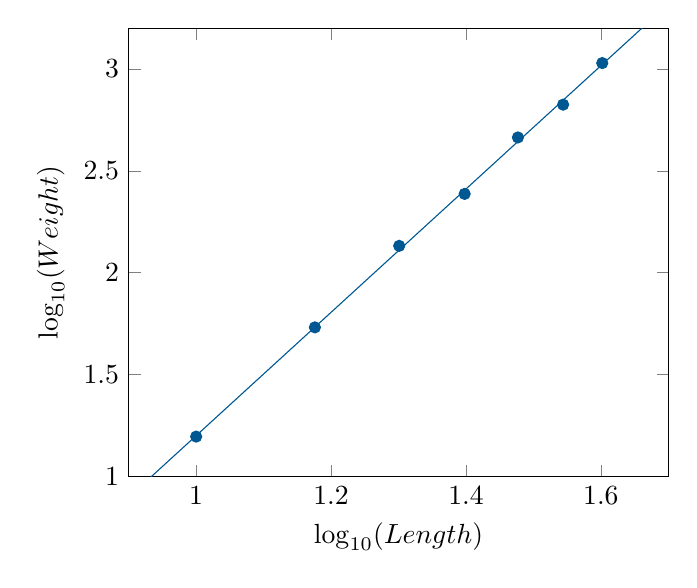
\begin{tikzpicture}
        \begin{axis}[
            xmin=0.9,xmax=1.7,
            ymin=1.0,ymax=3.2,
            xlabel={$\log_{10}(\text{Length})$},
            ylabel={$\log_{10}(\text{Weight})$},
        ]
        \addplot[only marks, mark size=2pt, kontinuablue] coordinates {(1.000,1.196)(1.176,1.732)(1.301,2.132)(1.398,2.387)(1.477,2.664)(1.544,2.825)(1.602,3.029)};
        \addplot[kontinuablue, domain=0.9:1.7, samples=2] {3.0258*x - 1.8251};
        \end{axis}
    \end{tikzpicture}
    \caption{The fish data after a log-log transformation. Both axes are logarithms, and the points fall along a line.}
    \label{fig:fishLog}
\end{figure}

Regressing $\log_{10}(y)$ on $\log_{10}(x)$ gives $\log_{10}(\hat{y}) = 3.0258\log_{10}(x) - 1.8251$, with $r = 0.9997$ and $r^2 = 0.9993$, a much tighter fit than the raw linear attempt.

The slope is $b$ itself, so $b \approx 3.026$. The intercept is $\log_{10}(a)$, so $a = 10^{-1.8251} \approx 0.01496$. That gives:
\[
\hat{y} = 0.01496 \cdot x^{3.026}
\]

An exponent close to 3 reflects real biology: fish grow in three dimensions at once, so weight scales close to the cube of length.

At $x = 45$ cm: $\log_{10}(\hat{y}) = 3.0258\log_{10}(45) - 1.8251 = 3.177$, so $\hat{y} \approx 10^{3.177} \approx 1{,}503.9$ g.

\begin{itemize}
    \item If $y = a \cdot x^b$, then $\log(y) = \log(a) + b\log(x)$, linear in $\log(x)$.
    \item Graphing $\log(y)$ against $\log(x)$, a \newterm{log-log plot}\index{log-log plot}, turns a genuine power relationship into a line.
    \item The transformed slope equals $b$ directly; the transformed intercept equals $\log(a)$.
    \item To predict $y$, find $\log(x)$ first, use the linear model to get $\log(\hat{y})$, then raise 10 to that power.
\end{itemize}

\begin{Exercise}[title={Fall Time}, label=fall_time]

A student drops a ball from different heights and times how long it takes to hit the ground:

\begin{table}[H]
\begin{tabular}{c|c}
Height, m ($x$) & Fall time, s ($y$) \\
\hline
5 & 1.01 \\
10 & 1.42 \\
15 & 1.71 \\
20 & 2.02 \\
25 & 2.24 \\
30 & 2.45 \\
35 & 2.59
\end{tabular}
\end{table}

\begin{enumerate}
    \item Explain why the shape of this scatterplot points to a power model rather than an exponential one.
    \item Regressing $\log_{10}(y)$ on $\log_{10}(x)$ gives $\log_{10}(\hat{y}) = 0.4908\log_{10}(x) - 0.3388$, with $r = 0.9996$. Use this to write the power model $\hat{y} = a \cdot x^b$.
    \item Predict the fall time from a height of $50$ m.
\end{enumerate}

\end{Exercise}
\begin{Answer}[ref=fall_time]

The raw scatterplot rises quickly at first and then levels off, growing more slowly as height increases. Exponential growth does the opposite: it starts slow and accelerates. That mismatch in shape is the signal to try a power model instead.

Slope $= b \approx 0.4908$. Intercept $= \log_{10}(a) = -0.3388$, so $a = 10^{-0.3388} \approx 0.4584$. The model is:
\[
\hat{y} = 0.4584 \cdot x^{0.4908}
\]

An exponent near 0.5 matches the physics: fall time under gravity is proportional to the square root of height, $t \propto \sqrt{h}$.

At $x = 50$: $\log_{10}(50) \approx 1.699$, so $\log_{10}(\hat{y}) = 0.4908(1.699) - 0.3388 = 0.495$, giving $\hat{y} \approx 10^{0.495} \approx 3.13$ s.

\end{Answer}

\section{Choosing the Right Transformation}

Both sections in this chapter start from the same move: something is curved, so take a logarithm and see if it straightens out. The two models call for a different logarithm, and mixing them up wastes time on a transformation that will not work.

\begin{table}[H]
\centering
\begin{tabular}{l|l|l|l}
Model & Equation & Transform & Linear in \\
\hline
Exponential & $y = a \cdot b^x$ & $\log(y)$ vs. $x$ & $x$ \\
Power & $y = a \cdot x^b$ & $\log(y)$ vs. $\log(x)$ & $\log(x)$
\end{tabular}
\end{table}

When you are unsure which model fits, try both transformations and compare. Graph $\log(y)$ against $x$: if that looks straight, the relationship is exponential. If it still curves, graph $\log(y)$ against $\log(x)$ instead; if that straightens out, it is a power model. Whichever transformation gives the higher $r^2$ with no leftover pattern in the residuals is the one that matches the data.

These two transformations show up often outside the classroom: population growth tends to follow an exponential pattern, while relationships like body mass and metabolic rate, or a planet's distance from the sun and its orbital period, tend to follow a power model.
